\chapter{Simulation Results}
\section{DC Analysis}
\begin{figure} [H]
\centering
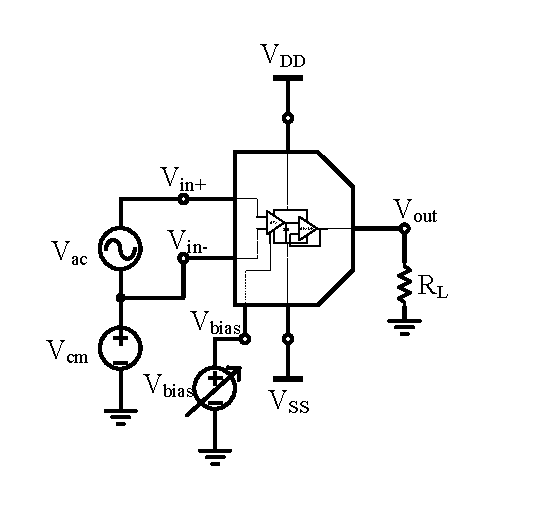
\includegraphics[scale=1]{Figures/Test_Benches/Overall/ACDC.pdf}
\caption{Test setup for DC Analysis}
\end{figure}

\begin{table} [H]
\centering
\begin{tabular}{@{}cc@{}}
\toprule
Vbias (mV)			& Output DC Bias (mV)	\\ \midrule
150					& 180.1  \\
200					& 148.4  \\
250					& 115.8  \\
300					& 82.28	 \\
350					& 47.83	 \\
400					& 12.45	 \\
450					& -23.86 \\
500					& -61.08 \\
550					& -99.24 \\
600					& -138.3 \\
650					& -178.4 \\
700 				& -219.3 \\
\bottomrule
\end{tabular}
\caption{DC Bias Point at the output of the circuit}
\end{table}


\section{AC Analysis}

\begin{figure} [H]
\centering
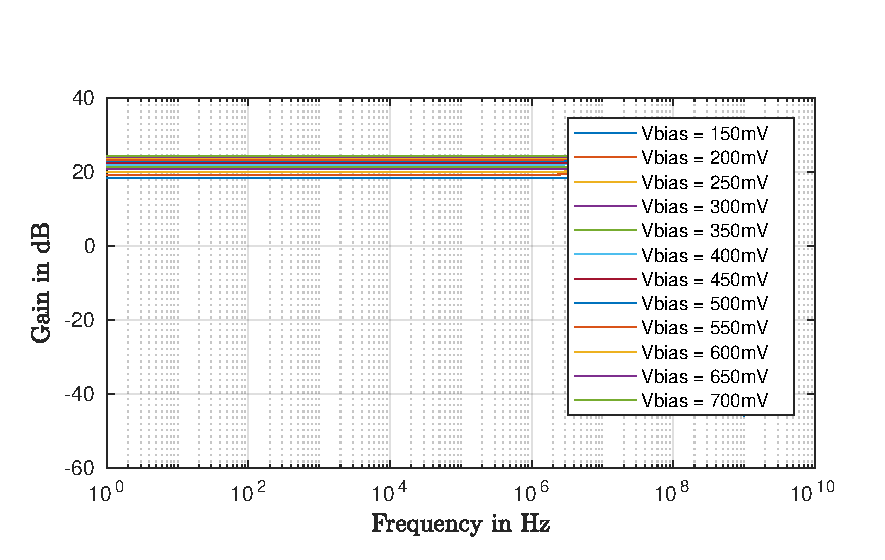
\includegraphics[scale=1]{Figures/Plots/Ov_Gain.pdf}
\caption{Plot of Gain vs Frequency for different Vbias}
\end{figure}

\begin{table} [H]
\centering
\begin{tabular}{@{}cccc@{}}
\toprule
Vbias (mV)			& DC Gain (dB) 	& Bandwidth (MHz) 	& Phase Margin \\ \midrule
150					& 18.5  		& 14.43 			& 55.49 \\
200					& 19.34			& 14.38 			& 51.37 \\
250					& 20.13  		& 14.34 			& 47.76 \\
300					& 20.83	 		& 14.29 			& 45.08 \\
350					& 21.46			& 14.24 			& 42.55 \\
400					& 22.02	 		& 14.19 			& 40.19 \\
450					& 22.52 		& 14.14 			& 38	\\
500					& 22.97 		& 14.08 			& 35.97	\\
550					& 23.38 		& 14.01 			& 34.08 \\
600					& 23.75 		& 13.95 			& 32.31 \\
650					& 24.1 			& 13.88 			& 30.63 \\
700 				& 24.43 		& 13.8  			& 29.02 \\
\bottomrule
\end{tabular}
\caption{DC Gain, Bandwidth and Phase Margin of the Overall System}
\end{table}

\begin{figure} [H]
\centering
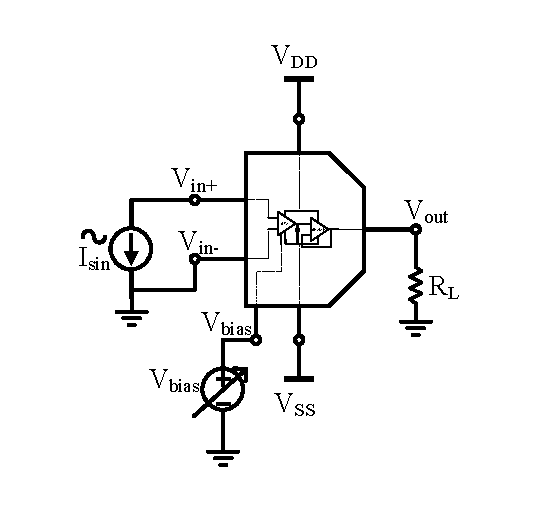
\includegraphics[scale=1]{Figures/Test_Benches/Overall/ZIN.pdf}
\caption{Test setup to measure Input Impedance}
\end{figure}

\begin{table} [H]
\centering
\begin{tabular}{@{}cc@{}}
\toprule
Vbias (mV)			& Input Impedance (Mega Ohms)	\\ \midrule
150					& 3.394  \\
200					& 3.402  \\
250					& 3.41   \\
300					& 3.418	 \\
350					& 3.425	 \\
400					& 3.433	 \\
450					& 3.44  \\
500					& 3.448 \\
550					& 3.456 \\
600					& 3.464 \\
650					& 3.473 \\
700 				& 3.482 \\
\bottomrule
\end{tabular}
\caption{Input Impedance of the Overall System}
\end{table}

\begin{figure} [H]
\centering
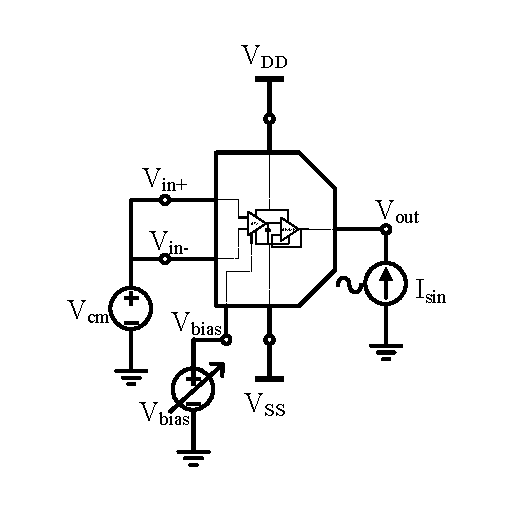
\includegraphics[scale=1]{Figures/Test_Benches/Overall/ZOUT.pdf}
\caption{Test setup to measure Output Impedance}
\end{figure}

\begin{table} [H]
\centering
\begin{tabular}{@{}cc@{}}
\toprule
Vbias (mV)			& Output Impedance (Ohms)	\\ \midrule
150					& 0.9415 \\
200					& 0.9434 \\
250					& 0.9453 \\
300					& 0.9474 \\
350					& 0.9495 \\
400					& 0.9517 \\
450					& 0.9541 \\
500					& 0.9565 \\
550					& 0.9591 \\
600					& 0.9618 \\
650					& 0.9646 \\
700 				& 0.9675 \\
\bottomrule
\end{tabular}
\caption{Output Impedance of the Overall System}
\end{table}

\begin{figure} [H]
\centering
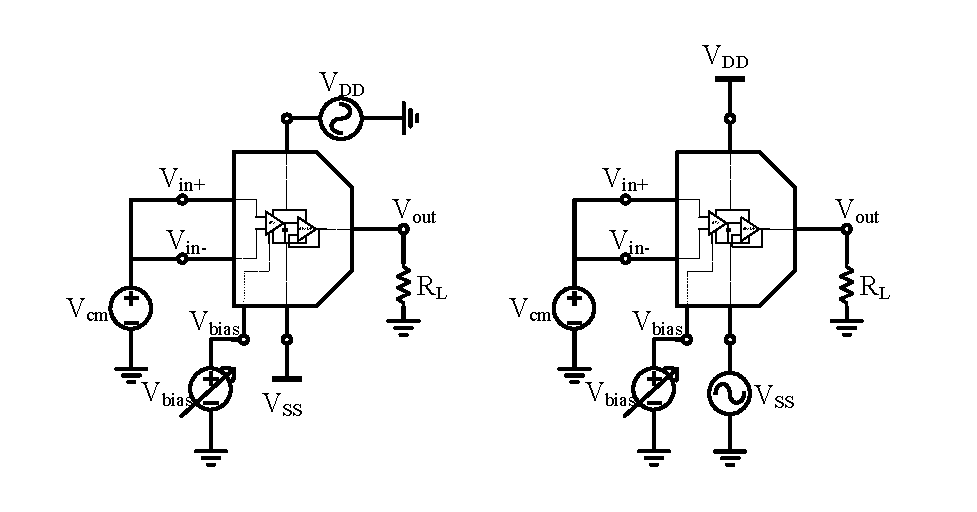
\includegraphics[scale=1]{Figures/Test_Benches/Overall/PSRR.pdf}
\caption{Test setup to measure PSRR}
\end{figure}

\begin{table} [H]
\centering
\begin{tabular}{@{}ccc@{}}
\toprule
Vbias (mV)			& PSRR (VDD)(uA/V)			& PSRR (VSS)(uA/V)	 \\ \midrule
150					& 97.76	 					& 93.69					 \\
200					& 89.66 					& 85.77					 \\
250					& 82.86 					& 79.11					 \\
300					& 77.26 					& 73.59					 \\
350					& 72.68						& 69.04					 \\
400					& 68.93						& 65.28					 \\
450					& 65.84 					& 62.18					 \\
500					& 63.27						& 59.53					 \\
550					& 61.1	 					& 57.26					 \\
600					& 59.22 					& 55.28					 \\
650					& 57.59 					& 53.52					 \\
700 				& 56.13 					& 51.92					 \\
\bottomrule
\end{tabular}
\caption{PSRR of the Overall System}
\end{table}

\section{Transient Analysis}
\begin{figure} [H]
\centering
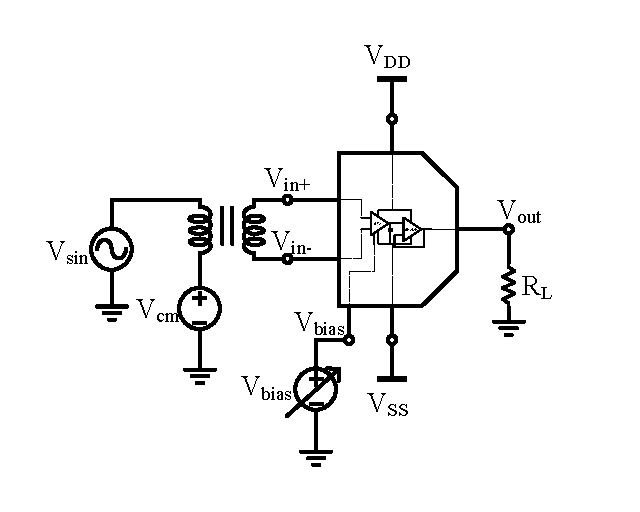
\includegraphics[scale=1]{Figures/Test_Benches/Overall/SINE.pdf}
\caption{Test setup for Transient Analysis - Sine Wave input}
\end{figure}

\begin{figure} [H]
\centering
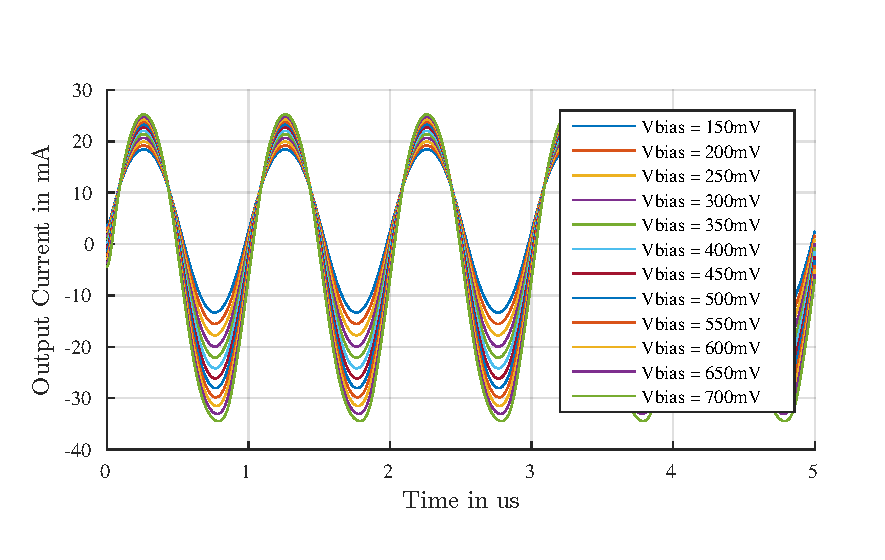
\includegraphics[scale=1]{Figures/Plots/Ov_Sine_Iout.pdf}
\caption{Plot of Output Current vs time for different Vbias}
\end{figure}

\begin{table} [H]
\centering
\begin{tabular}{@{}cccccc@{}}
\toprule
Vbias (mV)		& Iout Max(mA)		& Iout Min(mA)	 & Iout p2p (mA) & HD2 (dBc)	&HD3 (dBc) \\ \midrule
150				& 18.43	 			& -13.34		 & 31.77		& -37.14		& -48.17	\\
200				& 19.17 			& -15.55		 & 34.72		& -36.62		& -45.67	\\
250				& 19.93 			& -17.77		 & 37.7			& -35.65		& -43.65	\\
300				& 20.67 			& -19.97		 & 40.64		& -35.15		& -42.07	\\
350				& 21.38				& -22.12		 & 43.49		& -34.84		& -40.83	\\
400				& 22.04				& -24.19		 & 46.23		& -34.72		& -39.85	\\
450				& 22.66 			& -26.17		 & 48.83		& -34.8			& -39.01	\\
500				& 23.24				& -28.05		 & 51.29		& -35.08		& -38.24	\\
550				& 23.77	 			& -29.83		 & 53.6			& -35.54		& -37.42	\\
600				& 24.28 			& -31.51		 & 55.79		& -36.13		& -36.47	\\
650				& 24.76 			& -33.07		 & 57.83		& -36.61		& -35.24	\\
700 			& 25.24 			& -34.47		 & 59.71		& -36.44		& -33.61	\\
\bottomrule
\end{tabular}
\caption{Transient Parameters of the Overall System}
\end{table}

\begin{figure} [H]
\centering
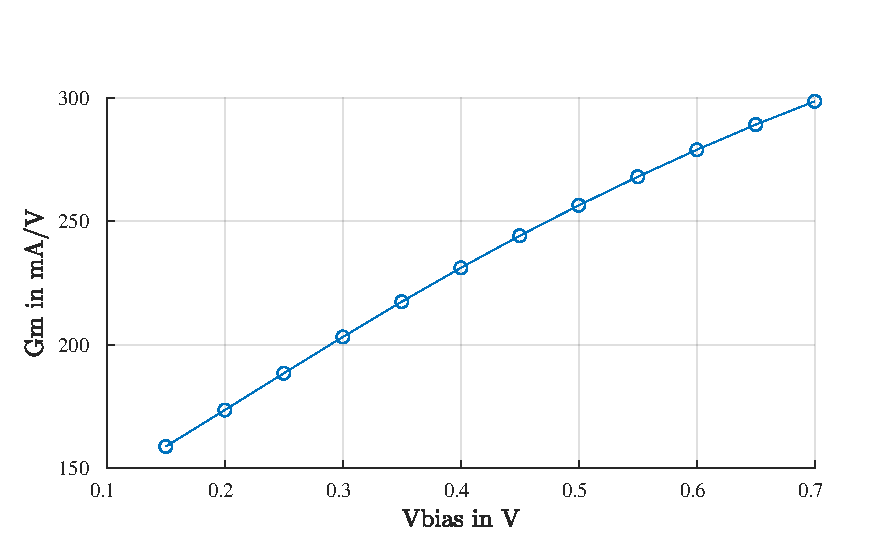
\includegraphics[scale=1]{Figures/Plots/Ov_Gm.pdf}
\caption{Plot of Gm vs Vbias}
\end{figure}

\begin{table} [H]
\centering
\begin{tabular}{@{}cc@{}}
\toprule
Vbias (mV)			& Transconductance (mA/V)	\\ \midrule
150					& 158.8 \\
200					& 173.6 \\
250					& 188.5 \\
300					& 203.2 \\
350					& 217.5 \\
400					& 231.2 \\
450					& 244.2 \\
500					& 256.4 \\
550					& 268 \\
600					& 278.9 \\
650					& 289.1 \\
700 				& 298.5 \\
\bottomrule
\end{tabular}
\caption{Transconductance Gain of the Overall System}
\end{table}

\begin{figure} [H]
\centering
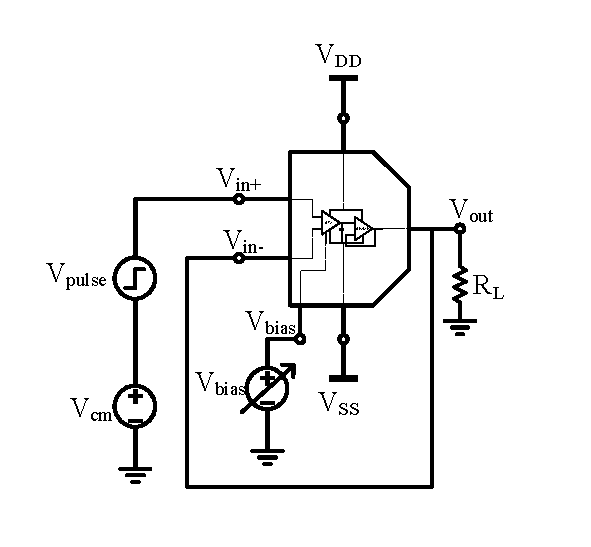
\includegraphics[scale=1]{Figures/Test_Benches/Overall/SLEW.pdf}
\caption{Test setup for Transient Analysis - Square Wave input}
\end{figure}

\begin{table} [H]
\centering
\begin{tabular}{@{}ccc@{}}
\toprule
Vbias (mV)			& Slew Rate (Rising Edge)(V/us)			& Slew Rate (Falling Edge)(V/us)	 \\ \midrule
150					& 6.985	 					& -8.73					 \\
200					& 7.505 					& -9.779				 \\
250					& 8.042 					& -10.68				 \\
300					& 8.581 					& -11.34				 \\
350					& 9.095						& -11.66				 \\
400					& 9.561						& -11.7					 \\
450					& 9.954 					& -11.6					 \\
500					& 10.27						& -11.45				 \\
550					& 10.49	 					& -11.3					 \\
600					& 10.65 					& -11.14				 \\
650					& 10.76 					& -10.99				 \\
700 				& 10.82 					& -10.84				 \\
\bottomrule
\end{tabular}
\caption{Slew Rate of the Overall System}
\end{table}

\section{Noise Analysis}

\begin{figure} [H]
\centering
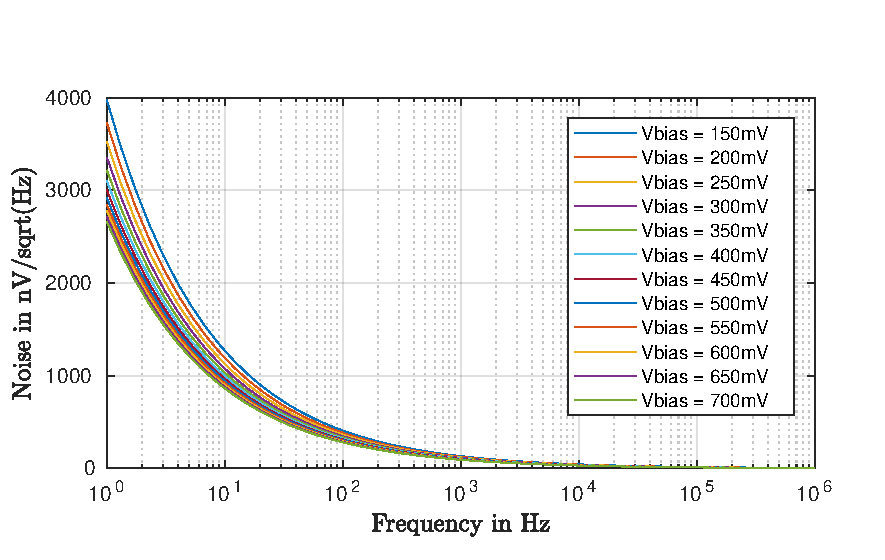
\includegraphics[scale=1]{Figures/Plots/Ov_Noise.pdf}
\caption{Plot of Input Referred Noise vs Frequency for different Vbias}
\end{figure}

\begin{table} [H]
\centering
\begin{tabular}{@{}cc@{}}
\toprule
Vbias (mV)			& Input Referred Noise (nV/sqrt(Hz))	\\ \midrule
150					& 46.64 \\
200					& 43.93 \\
250					& 41.71 \\
300					& 39.91 \\
350					& 38.46 \\
400					& 37.29 \\
450					& 36.33 \\
500					& 35.52 \\
550					& 34.82 \\
600					& 34.21 \\
650					& 33.66 \\
700 				& 33.16 \\
\bottomrule
\end{tabular}
\caption{Input Referred Noise of the Overall System}
\end{table}


\section{Programmable Load}

\begin{figure} [H]
\centering
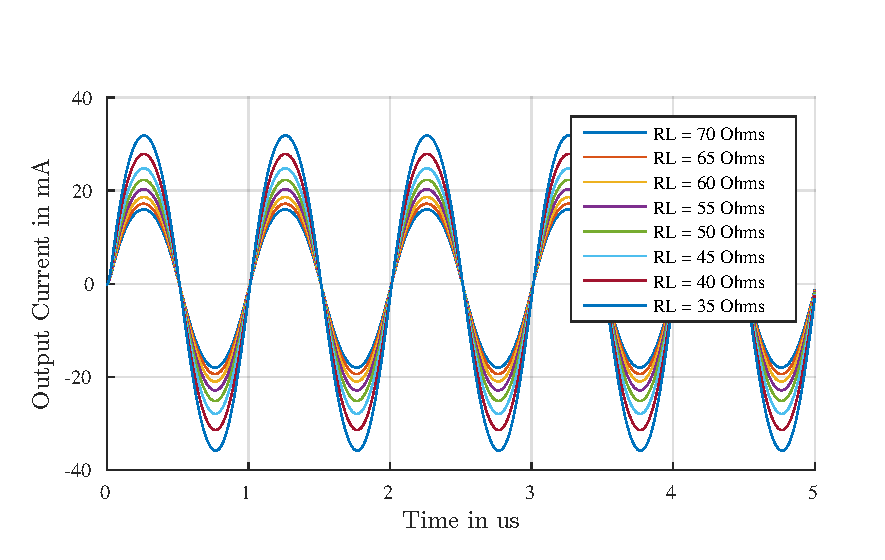
\includegraphics[scale=1]{Figures/Plots/Ov_Sine_RL.pdf}
\caption{Plot of Output Current vs Time for different RL}
\end{figure}

\begin{figure} [H]
\centering
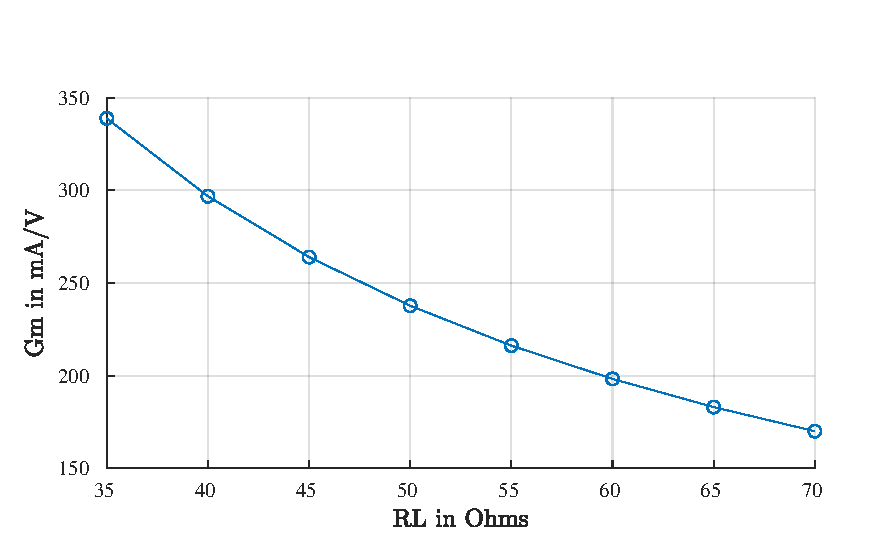
\includegraphics[scale=1]{Figures/Plots/Ov_Gm_RL.pdf}
\caption{Plot of Output Current vs time for different RL}
\end{figure}

\section{Corner Simulation}
\subsection{Process Variation}
\subsection{Process and Supply Variation}
\subsection{Process, Voltage and Temperature (PVT) variation}
\subsection{Summary of PVT Corner Analysis}